%% Standalone figure: compile this file once (pdflatex averaging.tex) to produce averaging.pdf,
%% which main.tex includes with \includegraphics. Recompile only after editing the figure.
\documentclass[11pt,tikz,border=2pt]{standalone}
\usepackage{amsmath,amssymb}       % \text, \vec, math symbols
\usetikzlibrary{arrows.meta}       % Stealth arrow tips
\begin{document}
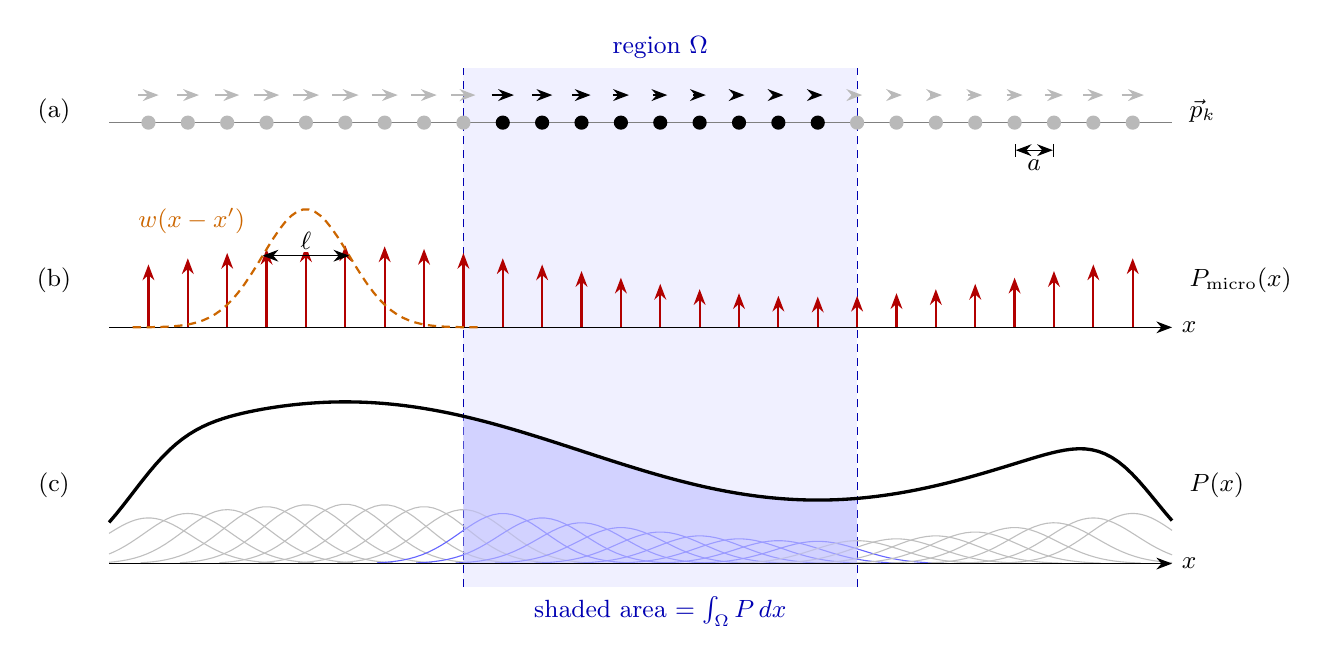
\begin{tikzpicture}[
  font=\small,
  >={Stealth[length=2mm]},
  declare function={
    spacing = 0.5;                                % interatomic distance a (cm)
    sig     = 0.55;                               % half-width of w (cm); width l ~ 2*sig
    pscale  = 1.3;                                % vertical plot scale of P(x)
    dip(\x) = 0.55 + 0.25*sin(deg(2*pi*\x/12));   % slowly varying dipole size p_k
  }
]
  % ---------- region Omega (spans all panels) ----------
  \def\xa{4.5}  \def\xb{9.5}
  \fill[blue!6] (\xa,-0.3) rectangle (\xb,6.3);
  \draw[densely dashed, blue!70!black] (\xa,-0.3) -- (\xa,6.3) (\xb,-0.3) -- (\xb,6.3);
  \node[blue!70!black] at ({(\xa+\xb)/2},6.55) {region $\Omega$};

  % ---------- (a) chain of atoms with dipoles ----------
  \node at (-0.7,5.75) {(a)};
  \draw[gray] (0,5.6) -- (13.5,5.6);
  \foreach \k in {1,...,26}{
    \pgfmathsetmacro{\xk}{\k*spacing}
    \pgfmathsetmacro{\len}{0.42*dip(\xk)}
    \pgfmathtruncatemacro{\inside}{(\xk>\xa) && (\xk<\xb)}
    \ifnum\inside=1 \def\col{black}\else\def\col{gray!55}\fi
    \fill[\col] (\xk,5.6) circle (0.09);
    \draw[->, thick, \col] ({\xk-\len/2},5.95) -- ({\xk+\len/2},5.95);
  }
  \draw[|<->|] (11.5,5.25) -- (12.0,5.25) node[midway, below] {$a$};
  \node[anchor=west] at (13.6,5.75) {$\vec p_k$};

  % ---------- (b) microscopic density and one averaging window ----------
  \node at (-0.7,3.6) {(b)};
  \draw[->] (0,3.0) -- (13.5,3.0) node[right] {$x$};
  \foreach \k in {1,...,26}{
    \pgfmathsetmacro{\xk}{\k*spacing}
    \draw[->, thick, red!70!black] (\xk,3.0) -- (\xk,{3.0+1.3*dip(\xk)});
  }
  % averaging window w centred at x' = 2.5
  \draw[thick, densely dashed, orange!80!black, domain=0.3:4.7, samples=60]
    plot (\x, {3.0 + 1.5*exp(-((\x-2.5)^2)/(2*sig^2))});
  \draw[<->] ({2.5-sig},{3.0+1.5*exp(-0.5)}) -- ({2.5+sig},{3.0+1.5*exp(-0.5)})
    node[midway, above=1pt, fill=white, inner sep=1pt] {$\ell$};
  \node[orange!80!black, anchor=east] at (1.85,4.35) {$w(x-x')$};
  \node[anchor=west] at (13.6,3.6) {$P_{\text{micro}}(x)$};

  % ---------- (c) smooth polarization ----------
  \node at (-0.7,1.0) {(c)};
  % build P(x) = sum_k p_k w(x - x_k) as one pgfmath expression
  \def\Psum{0}
  \foreach \k in {1,...,26}{
    \xdef\Psum{\unexpanded\expandafter{\Psum} + dip(\k*spacing)*exp(-((\noexpand\x-\k*spacing)^2)/(2*sig^2))}
  }
  \def\Pnorm{pscale/(sig*sqrt(2*pi))}   % normalization of w times the plot scale
  % individual contributions p_k w(x - x_k)
  \foreach \k in {1,...,26}{
    \pgfmathsetmacro{\xk}{\k*spacing}
    \pgfmathtruncatemacro{\inside}{(\xk>\xa) && (\xk<\xb)}
    \ifnum\inside=1 \def\col{blue!60}\else\def\col{gray!50}\fi
    \draw[\col, thin, domain={max(0,\xk-1.6)}:{min(13.5,\xk+1.6)}, samples=40]
      plot (\x, {\Pnorm*dip(\xk)*exp(-((\x-\xk)^2)/(2*sig^2))});
  }
  % area under P(x) inside Omega
  \fill[blue!25, opacity=0.6, domain=\xa:\xb, samples=60]
    (\xa,0) -- plot (\x, {\Pnorm*(\Psum)}) -- (\xb,0) -- cycle;
  \draw[very thick, domain=0:13.5, samples=160] plot (\x, {\Pnorm*(\Psum)});
  \draw[->] (0,0) -- (13.5,0) node[right] {$x$};
  \node[anchor=west] at (13.6,1.0) {$P(x)$};
  \node[blue!70!black, anchor=north] at ({(\xa+\xb)/2},-0.3) {shaded area $=\int_\Omega P\,dx$};
\end{tikzpicture}
\end{document}
